\chapter{Cơ sở lý thuyết}

\section {Kiến thức cơ bản về phishing }
Hiện tượng lừa đảo (phishing) lần đầu tiên được ghi nhận vào năm 1996
trong nhóm tin tức của hacker ~\cite{ollmann2004phishing}. Thuật ngữ "phishing" bắt nguồn từ từ "fishing" (câu cá), với việc thay thế chữ cái "f" bằng "ph" ~\cite{sunil2012pagerank}. Tài khoản người dùng có thông tin đăng nhập bị xâm phạm thường được gọi là lừa đảo (phishing), và người lấy được thông tin đăng nhập bị đánh cắp thành công được gọi là kẻ lừa đảo (phisher). Một trang web lừa đảo được thiết kế để bắt chước một trang web thật và đánh cắp thông tin nhạy cảm của người dùng để khai thác nó.Kẻ tấn công thường thao túng các thành phần hostname và đường dẫn của trang web mục tiêu để tạo ra một URL lừa đảo [19]. Thuật ngữ URL (Uniform Resource Locator) đề cập đến địa chỉ web xác định vị trí của một tài nguyên. Một tài nguyên web có thể bao gồm nhiều định dạng khác nhau, bao gồm trang web, tệp văn bản, email, hình ảnh và truy cập cơ sở dữ liệu [20]. Một URL bao gồm hai thành phần chính: định danh giao thức và đường dẫn tài nguyên.
\begin{figure}[htbp]
    \centering
    
    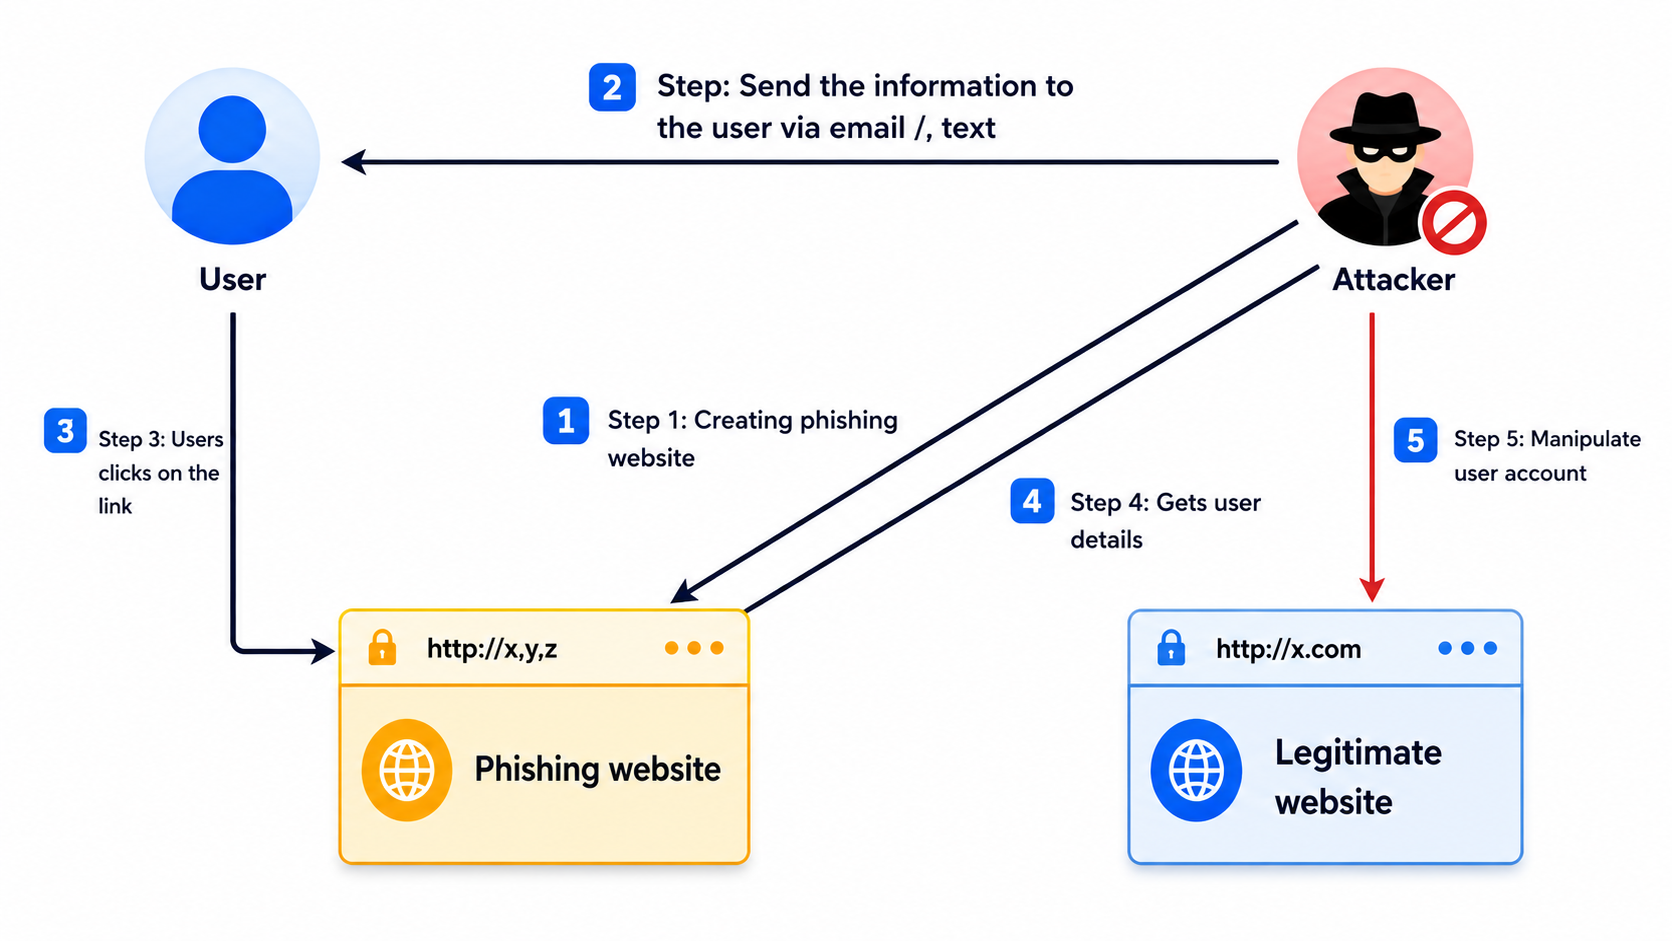
\includegraphics[width=0.9\textwidth]{figures/phishing cycle.png} 
    \caption{Cuộc tấn công lừa đảo điển hình.}
    \label{fig:phishing-cycle}
\end{figure}

Hình~\ref{fig:phishing-cycle}, cho thấy vòng đời của liên kết lừa đảo.Đầu tiên, một kẻ tấn công tạo ra một trang web lừa đảo giống với một trang web hợp pháp. Kẻ tấn công thao túng các yếu tố URL, chẳng hạn như tên miền và thư mục tài nguyên mạng, bằng cách đưa vào lỗi chính tả hoặc sử dụng các ký tự chữ cái tương tự để tạo một phiên bản sao chép của trang web hợp pháp. Ví dụ, URL "https://aimazon.az-z7acyu3z0y10.abc/m" sao chép hình thức và chức năng của trang web hợp pháp "https://www.amazon.com." Khi người dùng truy cập vào các trang web giả mạo, kẻ tấn công sẽ thu thập thông tin nhạy cảm để khai thác.

\section{Tiện ích Trình duyệt (Browser Extension)}

\subsection{Tổng quan}
Tiện ích trình duyệt là một chương trình có chức năng mở rộng ra thêm nhiều chức năng khác mà trình duyệt web cơ bản không cung cấp. Các tiện ích mở rộng này mang đến trải nghiệm lướt web tiện lợi, thông minh cho người dùng, thường được xây dựng dựa trên các công nghệ web tiêu chuẩn như HTML, CSS, JavaScript.

Trong lĩnh vực an ninh mạng, tiện ích trình duyệt có lợi thế quan trọng là khả năng truy cập trực tiếp vào nội dung của trang web mà người dùng đang tương tác. Nhờ đó, tiện ích có thể giám sát và phân tích dữ liệu theo thời gian thực, hỗ trợ phát hiện các hành vi hoặc nội dung độc hại.

\subsection{Kiến trúc tiện ích trình duyệt}
Kiến trúc của tiện ích hiện đại được xây dựng dựa trên tiêu chuẩn Manifest V3 nhằm đảm bảo hiệu năng và tính bảo mật~\cite{ref9}. Các thành phần chính bao gồm:

\begin{itemize}
    \item Tệp kê khai manifest.json: Tệp cấu hình chứa siêu dữ liệu xác định quyền hạn quyền, khai báo thành phần.và phạm vi hoạt động của tiện ích
    
    \item Tập lệnh nền (Content Scripts.js): Thành phần được chèn vào trang web để truy cập và xử lý nội dung DOM  để tìm các liên kết.
    
    \item Background Scripts (Service Workers): Thành phần xử lý trung tâm, thực hiện giao tiếp với mô hình AI và điều phối dữ liệu.
    
    \item Pop-up UI: Giao diện người dùng hiện thị kêt quả phân tích cho người dùng.
    
\end{itemize}

\subsection{Cơ chế hoạt động }
Trong bài toán phát hiện phishing, tiện ích trình duyệt không chỉ kiểm tra trang web hiện tại mà còn quét các liên kết xuất hiện trong nội dung trang như bài đăng, bình luận hoặc email.

Quy trình hoạt động bao gồm:
\begin{enumerate}
    \item Content script có nhiệm vụ thu thập các liên kết từ DOM trong các thẻ <a>.
    \item Dữ liệu khi quá thời gian 600ms không tìm liên kết mới được gom hết gửi đến background script để gửi sang cho server để xử lý.
    \item Những liên kết nhận được, đưa vào mô hình AI để phân loại dự đoán phishing. gom lại và trả về cho background gửi về cho content-script để làm hightlight đường dẫn và popup hiển thị cảnh báo cho người dùng.
\end{enumerate}


% =====================================================================
\subsection{Kỹ thuật giám sát và trích xuất dữ liệu Web động}
\label{sec:dynamic-web-extraction}

Trong các nền tảng mạng xã hội hiện đại, dữ liệu không được tải tĩnh mà được cập nhật liên tục thông qua quá trình cuộn trang. Điều này đặt ra thách thức cho việc phát hiện phishing theo thời gian thực.

 Mutation Observer là một API Web được cung cấp bởi các trình duyệt hiện đại để phát hiện các thay đổi trong DOM để theo dõi các thay đổi trong DOM theo thời gian thực. Khi một bài đăng mới trong trang được thêm vào danh sách hiển thị, trình duyệt sẽ tạo ra một MutationRecord. Tiện ích sẽ lọc các bản ghi này để xác định:
\begin{enumerate}
    \item \textbf{childList:} Theo dõi các phần tử con mới được thêm vào (thường là các thẻ \texttt{<div>} chứa bài đăng).
    \item \textbf{subtree:} Cho phép theo dõi toàn bộ các cấp con bên trong để đảm bảo không bỏ sót các liên kết thẻ \texttt{<a>} nằm sâu trong cấu trúc bài viết.
\end{enumerate}
Quy trình này giúp hệ thống chỉ thực hiện quét khi có dữ liệu mới, tối ưu hóa hiệu năng và đảm bảo tính ổn định của trình duyệt.


% =====================================================================
\section{Cơ sở lý thuyết về Học máy trong Phát hiện Phishing}
\label{sec:classification-mechanism}

\subsection{Thuật toán XGBoost (Extreme Gradient Boosting)}
Thuật toán XGBoost là một phương pháp học kết hợp (Ensemble Learning) dựa trên kỹ thuật tăng cường độ dốc (Gradient Boosting). Khác với Random Forest (xây dựng các cây độc lập), XGBoost xây dựng các cây quyết định một cách tuần tự, trong đó mỗi cây sau cố gắng sửa chữa những sai lầm của các cây trước đó.
\begin{enumerate}
    \item \textbf{Tối ưu hóa hàm mục tiêu:} XGBoost sử dụng chuỗi xấp xỉ Taylor bậc hai để tối ưu hóa hàm mất mát, giúp quá trình hội tụ diễn ra nhanh chóng và chính xác.
    \item \textbf{Kiểm soát quá khớp (Overfitting):} Thuật toán tích hợp các thành phần chính quy hóa (L1, L2 regularization) trực tiếp vào hàm mục tiêu, giúp mô hình ổn định với dữ liệu nhiễu.
    \item \textbf{Hiệu suất thực thi:} XGBoost được tối ưu hóa ở mức phần cứng, hỗ trợ tính toán song song, giúp thời gian suy luận cực ngắn, đặc biệt phù hợp cho ứng dụng thời gian thực như tiện ích trình duyệt.
\end{enumerate}

\subsection{Rò rỉ dữ liệu (Data Leakage) trong học máy}
Data Leakage là một lỗi nghiêm trọng trong việc huấn luyện mô hình học máy, xảy ra khi mô hình vô tình được học từ những thông tin (đặc trưng) mà trong thực tế nó không thể biết trước tại thời điểm dự đoán. Trong Cybersecurity, điều này dẫn đến độ chính xác cao giả tạo (ví dụ 100\%) khi huấn luyện, nhưng lại hoạt động rất tệ khi triển khai thực tế.
\begin{itemize}
    \item \textbf{Target Leakage (Rò rỉ nhãn):} Sử dụng các đặc trưng như \textit{URLSimilarityIndex} (yêu cầu biết trước tên miền gốc của nạn nhân) để dự đoán.
    \item \textbf{Collection Bias (Thiên lệch thu thập):} Các trang phishing thường tồn tại rất ngắn và bị sập. Khi công cụ thu thập dữ liệu tải trang, nó chỉ nhận được lỗi 404 với mã nguồn cực kỳ ngắn. Mô hình sẽ học cách nhận diện "trang web đã chết" thay vì "trang web lừa đảo".
\end{itemize}

\subsection{Khoảng cách Levenshtein (Phát hiện Typosquatting)}
Kỹ thuật tấn công Typosquatting (đăng ký tên miền cố tình viết sai chính tả, ví dụ \texttt{g00gle.com} thay vì \texttt{google.com}) rất phổ biến. Khoảng cách Levenshtein là thước đo số lượng thao tác chỉnh sửa tối thiểu (chèn, xóa, hoặc thay thế một ký tự) cần thiết để biến đổi chuỗi này thành chuỗi khác. Kỹ thuật Heuristic sử dụng khoảng cách này để so sánh tên miền hiện tại với danh sách các thương hiệu nổi tiếng, giúp nhận diện lừa đảo trực tiếp mà không phụ thuộc hoàn toàn vào AI.

\subsection{Hiệu chuẩn xác suất (Probability Calibration)}
Các mô hình cây quyết định thường trả về một điểm phân loại (score) không đại diện cho xác suất thực sự. Ví dụ, điểm 0.8 không có nghĩa là 80\% khả năng trang đó là phishing. Kỹ thuật \textbf{Isotonic Regression} được áp dụng để hiệu chuẩn lại điểm số này, đảm bảo xác suất đầu ra ánh xạ sát nhất với tỷ lệ phân phối thực tế của nhãn, giúp thiết lập các ngưỡng chặn (Thresholds) an toàn và đáng tin cậy.

\subsection{Khả năng giải thích AI (Explainable AI - SHAP)}
SHAP (SHapley Additive exPlanations) là phương pháp thuộc lĩnh vực XAI, dựa trên lý thuyết trò chơi hợp tác. Thuật toán \textit{TreeExplainer} của SHAP giúp giải mã cơ chế "hộp đen" của XGBoost bằng cách lượng hóa chính xác mức độ đóng góp của từng đặc trưng vào quyết định cuối cùng. Trong khóa luận này, SHAP được dùng để tự động trích xuất các "Cờ đỏ" (Red flags) nhằm giải thích cho người dùng lý do một trang web bị cảnh báo.

\subsection{Độ đo đánh giá trong bài toán An ninh mạng}
Trong bài toán phát hiện phishing, khóa luận tập trung tối ưu hóa sự cân bằng giữa rủi ro bảo mật và trải nghiệm người dùng thông qua chỉ số $F_{\beta}$ (với $\beta = 0.5$):
\begin{itemize}
    \item \textbf{False Positive (FP - Dương tính giả):} Chặn nhầm trang sạch. Yếu tố này phải được triệt tiêu để không làm gián đoạn người dùng.
    \item \textbf{False Negative (FN - Âm tính giả):} Bỏ sót trang phishing. Cần giữ ở mức tối thiểu.
    \item \textbf{Brier Score:} Đánh giá độ chính xác của điểm xác suất dự đoán sau khi hiệu chuẩn (càng gần 0 càng tốt).
\end{itemize}